
\section{Marco Te\'orico}
\label{sec:marcoteorico}

\subsection{Tecnolog\'ias en redes fot\'onicas}
\label{sec:redfotonica}

\subsubsection{Fibra de tipo G.652.D}

Como ya se ha dicho en secciones previas, la fibra oscura de la que se
dispone en el tendido preexistente es del tipo G.652.D. Sus
características ópticas se muestran en la tabla \ref{fig:tablafibra}.

\begin{figure}[H]
  \centering
  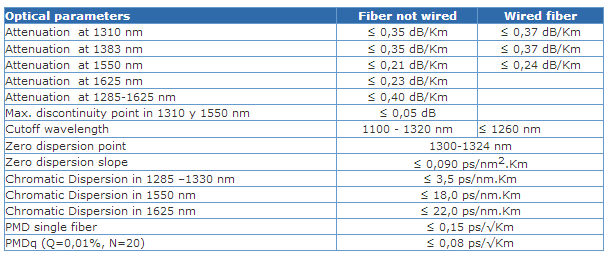
\includegraphics[scale=1]{Imagenes/Fibra.png}
  \caption{Carácteristicas ópticas fibra G.D652.D \cite{datasheetfibra}}
  \label{fig:tablafibra}
\end{figure}
  
Es sabido el hecho de que las fibras ópticas son muy susceptibles a
los factores medioambientales, siendo dentro de los más sensibles la
penetración de agua, vibración, cambios de temperatura y ataques
biológicos (e.g. roedores). También afectan para tendidos
aéreos las cargas de viento y hielos.

\subsubsection{DWDM}
\label{sec:dwdm}

Las redes de fibra óptica modernas utilizan una tecnología de
transporte de alta capacidad llamada \emph{Dense Wavelength Division
Multiplexing} (\emph{DWDM} o en español \emph{multiplexación densa de 
longitud de onda}). Esta tecnología permite introducir varias señales 
con distinta frecuencia a una misma fibra óptica mono modo, permitiendo 
transmisiones con mayores anchos de banda.\cite{dwdm1}\cite{dwdm2}

\emph{DWDM} opera en la capa de red, por lo que es independiente de
los protocolos de transporte y enlace. La multiplexación ocurre sobre
la banda C, es decir, a partir de la longitud de onda 1529,16 nm y
hasta 1560,61 nm ($\lambda$ central = 1510 nm). En frecuencias, esto
corresponde al rango entre 192100 GHz y 196000 GHz (frecuencia
central: 1931000 GHz).

A medida que aumentan los avances tecnológicos, los módulos que
trabajan con esta técnica de multiplexación incorporan mayor capacidad
al condensar cada vez más los canales en el espacio de frecuencia,
aumentando la cantidad de señales en una sola fibra. En la actualidad,
la mayor parte de las empresas de telecomunicaciones realiza diseños
que consideran espaciamientos de 100 o 50 GHz, lo que se traduce en
enlaces de 40 ú 80 canales (o $\lambda$'s) respectivamente. No
obstante, la ciencia ya experimenta con canales espaciados por 25 e
incluso 12,5 GHz solamente, pudiendo llegarse a incorporar en el
futuro hasta 320 $\lambda$ en una sola fibra. 

En la jerga de telecomunicaciones ópticas, a los distintos $\lambda$
se les llama también ``colores'', por la similitud de conceptos en la
óptica de comunicaciones y la óptica tradicional.

\begin{figure}[H]
  \centering
  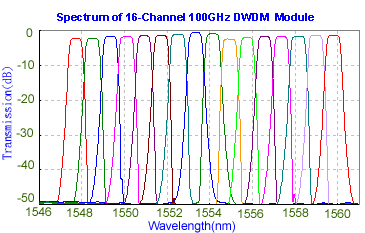
\includegraphics[scale=1]{Imagenes/DWDM_channels.png}
  \caption{Representación en el espacio frecuencial de distintas
    señales multiplexadas sobre la banda C utilizando DWDM.\cite{bandasdwdm} Se
    observan 16 canales de los 40 disponibles con un espaciamiento de
    100 GHz.}
  \label{fig:dwdmchannels}
\end{figure}

\subsubsection{OADM}
\label{sec:oadm}

Los dispositivos que se encargan de agregar o quitar $\lambda$'s de la
fibra con el fin de controlar el enlace por donde se encausan las
señales a enviar se llaman \emph{OADM}, siglas de ``optical add-drop
multiplexer''.

Existen dos tipos de \emph{OADM}. El más primitivo es el \emph{FOADM},
donde la F significa ``fixed'', es decir, fijo o estático. Este tipo
de direccionamiento no es reconfigurable, es decir, el diseño de la
red debe incluir los dispositivos que harán el encausamiento en los
nodos requeridos, sin permitir cambio dinámico de canales en la
fibra. En \emph{FOADM}, los filtros o LASER debían ser fijados en los
nodos, acorde a las necesidades de la red al momento de su diseño. En
el caso de requerir un cambio en la red se debían cambiar y reconectar
jumpers, debiendo detener el funcionamiento de la red por el tiempo
que este proceso demorase. Además, la granularidad o precisión del
encausamiento era de por lo menos $2\lambda$, lo cual introducía
despilfarro de recursos en la red, disminuyendo el ancho de banda de
la red a al menos la mitad.

Debido a este inconveniente, se creó y rápidamente se reemplazó el
\emph{FOADM} por el \emph{ROADM}, con la R de
``reconfigurable''. Estos dispositivos son reprogramables remotamente,
e incluso la conmutación puede cambiar de acuerdo a la demanda de
forma dinámica y automática. Su granularidad es de tan solo
$1\lambda$, convirtiéndose en la única opción realmente factible y
adecuada para diseñar redes escalables en el tiempo.

Los dispositivos \emph{ROADM} han evolucionado desde su primera
incorporación al mercado\cite{roadmevolves}. En un principio, los 
\emph{ROADM} debían realizar demultiplexación y multiplexación de
todos los canales para poder manejar eficientemente las señales,
además de varios otros inconvenientes. Esto elevaba notablemente el 
costo de la red pues para minimizar las pérdidas en los nodos se 
debían utilizar transpondedores de mejor calidad.

Los \emph{ROADM} de segunda generación mejoraban en algo los problemas
en la calidad de señal y permitían un switching de mayor calidad para
longitudes de onda individuales utilizando ``Wave Blocking'' (\emph{WB})
o bloqueo de onda. El \emph{WB} solucionaba varios de los problemas que
tenían los dispositivos \emph{ROADM} de primera generación, pero aún no
eran lo suficientemente robustos, pequeños y útiles para ser utilizados
a todo nivel, siendo las redes con \emph{ROADM} de segunda generación 
usualmente utilizadas sólo a nivel de redes metropolitanas.

La tercera generación de \emph{ROADM} hace uso de unos módulos
llamados \emph{WSS} (\emph{wavelength selective switch}). Esta
especificación introduce la capacidad de hacer redes totalmente
flexibles, de forma dinámica y sin necesidad de tener a técnicos
capacitados en la configuración de redes con \emph{OADM} fijos. 
Adicionalmente a la mejora tecnológica, los precios de los
dispositivos disminuyeron puesto al gran aumento de la oferta de
soluciones \emph{DWDM} integrados con \emph{ROADM}.

Otra de las bondades que trajo la introducción de los \emph{WSS} fue
haber incorporado la funcionalidad para interconectar redes de
distintas topologías (redes en anillo y redes en malla, por
ejemplo).

Las funcionalidades actuales de un \emph{ROADM} con \emph{WSS} son las
siguientes:
\begin{itemize}
\item \textbf{Add}: añade una señal externa a la red existente DWDM
\item \textbf{Drop}: extrae una señal de la red en el nodo donde se ejecuta la
  acción
\item \textbf{Switch}: se configura un nodo para unir dos redes y poder
  encausar el $\lambda$ a un nodo de otra red
\item \textbf{Pass-through}: se configura un nodo para no alterar a un
  $\lambda$
\end{itemize}

\subsubsection{Compensadores de atenuación}
\label{sec:amplificadores}

Se utilizan amplificadores ópticos para evitar la excesiva atenuación
de señal en el nodo de destino. Los amplificadores se clasifican según
su ubicación en el enlace\cite{G663}.

El \textbf{booster amplifier} es un dispositivo que se inserta 
directamente después del transmisor óptico. Es especialmente útil en
aplicaciones donde los \emph{OLA} o amplificadores intermedios no se
pueden y/o quieren insertar por algún motivo de diseño (e.g. redes 
submarinas). El ruido que insertan es despreciable, pero una mayor 
potencia a su salida repercute en distorsiones no lineales de la fibra
óptica. En ocasiones, los transmisores incluyen uno de estos
amplificadores.

El \textbf{preamplificador} va en el receptor y sirve para mejorar la
lectura de la señal por parte del dispositivo óptico de destino. En 
ocasiones, éste puede ir en el mismo módulo del receptor.

Los \textbf{optical line amplifiers} o amplificadores de línea sirven para
aumentar la potencia de forma de poder abarcar distancias de hasta miles
de kilómetros. Demasiados \emph{OLA} pueden aumentar el efecto de la
dispersión cromática no lineal y, sobre todo, aumentar los niveles de
ruido a niveles inmanejables, deteriorando demasiado el servicio de
distribución.

Todos los amplificadores pueden diseñarse de forma que el ruido que
inserten sea lo más acotado posible. Ello se logra introduciendo
filtros pasa banda adecuados a los diseños. Habiendo buenos
estándares, los filtros pueden ser diseñados de forma óptima para
casos generales.

La tecnología actual más típica de amplificadores aprovecha un
fenómeno físico del erbio ($Er_{68}$) que, al ser utilizado como
material dopante de fibra óptica y en presencia de una bomba de
fotones, amplifica la señal completa e introduce un ruido altamente
predecible y lineal. Estos amplificadores se llaman por sus siglas en
inglés \emph{EDFA} (\emph{Erbium Doped Fiber Amplifier}).

En este diseño solamente se usaron amplificadores booster y
preamplificadores, ya que las distancias de los enlaces no eran
suficientemente largas para introducir amplificadores de línea.

\subsubsection{Compensadores de dispersión}
\label{sec:dispersion}

La dispersión cromática es un efecto indeseable en las redes fotónicas
multicanal como lo es, en particular, la tecnología \emph{DWDM}. La
disepersión provoca que una señal se ensanche en el dominio de la
frecuencia (o lo que es lo mismo, que se afine en el dominio del
tiempo), haciendo que sea más probable la interferencia entre
$\lambda$'s de distintos canales. Afortunadamente, este fenómeno está
ampliamente estudiado y se sabe con bastante precisión cómo reducir su
efecto a un mínimo, al menos en su componente lineal, predominante en
señales con intensidades ``pequeñas''.

Existen dos enfoques para combatir la dispersión cromática lineal. Uno
es usando \emph{DSP} (procesamiento digital de señales) y el otro
usando dispositivos \emph{DCM} (dispersion compensation module). El
más relevante de estos enfoques y el más utilizado es el \emph{DCM}.

Todas las fibras ópticas tienen un coeficiente de dispersión cromática
que las caracteriza. El coeficiente depende de $\lambda$ y sus
unidades son $\frac{ps}{nm \times Km}$. Los \emph{DCM} son
dispositivos que se especifican en el mercado de acuerdo a su
distancia de fibra a compensar. Tienen un coeficiente de dispersión
negativo que contrarresta el efecto de la fibra en cuanto a la
dispersión que ella intrínsecamente provoca en la señal.

Además del efecto lineal de la dispersión, existen efectos no lineales
que se suman y que son muchísimo más complicados de compensar. Estos
son la \emph{SPM} (self phase modulation) y \emph{XPM} (cross phase
modulation). Estos efectos se producen ya que el campo eléctrico se
modula a sí mismo a medida que avanza en la fibra (cuando éste es lo
suficientemente grande, los efectos de \emph{SPM} y \emph{XPM} toman
mayor importancia).

\subsection{Dispositivos presentes en una red fotónica}
\label{sec:dispositivos}

A continuación se presenta un resumen de los elementos esenciales para
una red óptica basada en DWDM. Estos componentes llevan a la práctica
las tecnologías nombradas en la sección anterior.

\begin{itemize}
\item \textbf{Transpondedor}: ermite transformar una señal de
  algún protocolo de transporte típico (e.g. señales eléctricas) en
  ondas transmitibles por \emph{FO} (señales ópticas) y vice versa.
\item \textbf{Multiplexor/Demultiplexor}: los multiplexores permiten
  combinar señales con distinta longitud de onda provenientes de 
  entradas independientes y enviarlas por una salida común. Los
  demultiplexores hacen lo inverso; seleccionan una de las longitudes
  de onda de la entrada única y la transmiten a una salida individual.
\item \textbf{Amplificadores Ópticos}: mencionados en la sección 
  anterior, restauran la señal a un nivel apropiado para su uso en
  los componentes de la red (e.g. transporte por fibra, conmutación, 
  multiplexación y demultiplexación).
\item \textbf{Canal Óptico de Servicio}: este canal se ubica en una
  frecuencia fuera de la banda C estándar (1510 nm, nominalmente
  hablando). Sirve para transportar señales de alarma entre los
  componentes internos de la red (e.g. conmutadores).
\end{itemize}